\let\negmedspace\undefined
\let\negthickspace\undefined
\documentclass[journal,12pt,twocolumn]{IEEEtran}
\usepackage{cite}
\usepackage{amsmath,amssymb,amsfonts,amsthm}
\usepackage{algorithmic}
\usepackage{graphicx}
\usepackage{textcomp}
\usepackage{caption}
\usepackage{xcolor}
\usepackage{txfonts}
\usepackage{listings}
\usepackage{enumitem}
\usepackage{mathtools}
\usepackage{gensymb}
\usepackage[breaklinks=true]{hyperref}
\usepackage{tkz-euclide} % loads  TikZ and tkz-base
\usepackage{listings}
\usepackage{gvv}
\newtheorem{theorem}{Theorem}[section]
\newtheorem{problem}{Problem}
\newtheorem{proposition}{Proposition}[section]
\newtheorem{lemma}{Lemma}[section]
\newtheorem{corollary}[theorem]{Corollary}
\newtheorem{example}{Example}[section]
\newtheorem{definition}[problem]{Definition}
%\newtheorem{thm}{Theorem}[section] 
%\newtheorem{defn}[thm]{Definition}
%\newtheorem{algorithm}{Algorithm}[section]
%\newtheorem{cor}{Corollary}
\newcommand{\BEQA}{\begin{eqnarray}}
\newcommand{\EEQA}{\end{eqnarray}}
\newcommand{\define}{\stackrel{\triangle}{=}}
\theoremstyle{remark}
\newtheorem{rem}{Remark}

%\bibliographystyle{ieeetr}
\begin{document}
%

\bibliographystyle{IEEEtran}


\vspace{3cm}

\title{
%	\logo{
GATE MA-28(2022) 

\large{EE:1205-Signals and Systems}

Indian Institute of Technology, Hyderabad
%	}
}
\author{Md Ayaan Ashraf

EE23BTECH11041
}	

\maketitle

\newpage

%\tableofcontents

\bigskip
\renewcommand{\thefigure}{\arabic{figure}}
\renewcommand{\thetable}{\arabic{table}}
\section*{\textit{\textbf{Question}}}
The radius of convergence of the series
\begin{align}
    \sum_{n=0}^{\infty} 3^{n+1}z^{2n}, \quad z \in \mathbb{C} \nonumber{}
\end{align}is ?

\hfill {(GATE MA-28 (2022))}
\section*{\textit{\textbf{Solution:}}}

\begin{table}[h]
  \centering
  \begin{tabular}{|c|c|c|}
    \hline
Parameter & Description & Value \\ \hline
$x(n)$ & General Term & $3^{n+1}z^{2n}$\\
\hline
$Y(z)$ & Given Sum & $\sum_{n=0}^{\infty} 3^{n+1}z^{2n}, \quad z \in \mathbb{C} $\\
\hline
  \end{tabular}
  \vspace{2mm}
  \caption{GATE MA-28(2022)}
\end{table}




\begin{align}
x(n) =& 3\sum_{n=0}^{\infty} 3^{n}z^{2n}, \quad z \in \mathbb{C}\\
=&3\sum_{n=0}^{\infty} {(3z^{2})}^{n}\\
=&\frac{3}{1-3z^{2}}\\
    =& \frac{3}{(1-\sqrt{3}z)(1+\sqrt{3}z)}\\
    =& \frac{3}{2} \left(\frac{1}{1-\sqrt{3}z}+\frac{1}{1+\sqrt{3}z}\right)\\
    =&\frac{3}{2}\left(\frac{z^{-1}}{z^{-1}-\sqrt{3}}+\frac{z^{-1}}{z^{-1}+\sqrt{3}}\right)\\
    =&\frac{3}{2}\left(1- \frac{\sqrt{3}}{\sqrt{3}-z^{-1}}+1 -\frac{\sqrt{3}}{z^{-1}+\sqrt{3}}\right)\\
    \end{align}
     $\therefore$ For inverse Z transform,
     \begin{align}
    \implies \frac{3}{2}\left(2\delta(n)+ \left(\frac{1}{\sqrt{3}}\right)^n - \left(\frac{-1}{\sqrt{3}}\right)^n\right)
\end{align}  

 For Radius of Convergence,
 \begin{align}
|3z^2| < 1\\
|z| < \frac{1}{\sqrt{3}}
 \end{align}
 \begin{figure}[h]
\renewcommand\thefigure{1}
    \centering
    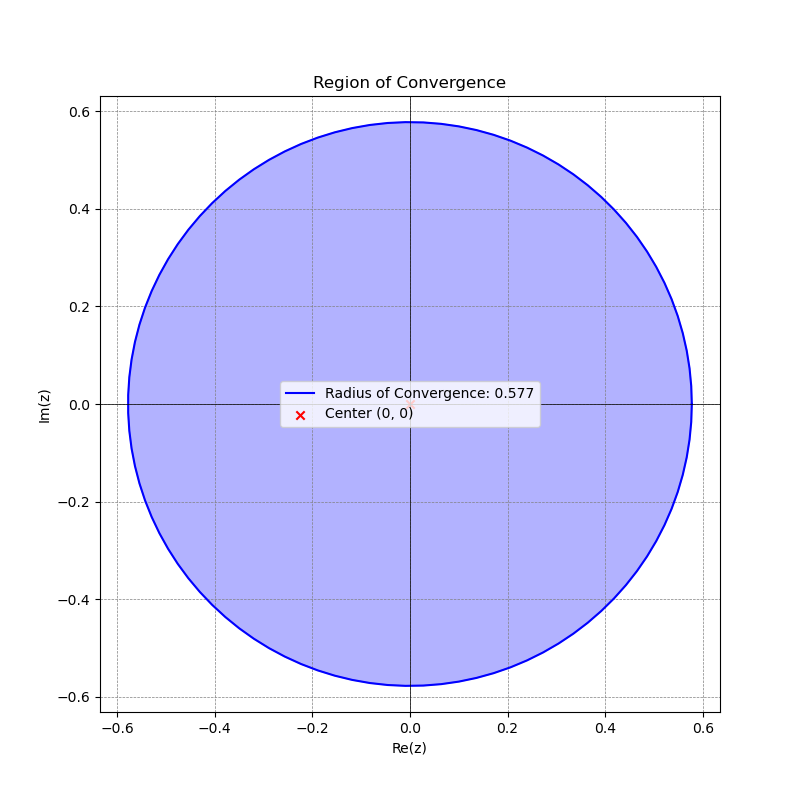
\includegraphics[width=0.8\columnwidth]{figs/fig1.png}
    \caption{ROC - $|z|< \frac{1}{\sqrt{3}}$}
    \label{Fig1_GATE MA 28}
\end{figure}
\end{document}

